\section{Semantic Segmentation with CNN}
\label{sec:network}
This section presents the architecture of the convolutional neural network, as well as the details surrounding the optimization and regularization of the network. 

\subsection{Patch-based Approach}
This thesis formulates the problem of road segmentation in aerial images in the same manner as \cite{Mnih_roads_high_res_aerial_images} did. This patch-based approach is presented in detail in Section \ref{sec:related_works}. In short, the convolutional neural network should learn the label distribution:

$$ p(m|s) = \prod_{i=0}^{w_m^2}p(m_i | s),  $$

\noindent where $p(m|s)$ denote a conditional probability of a label map patch given an aerial image patch. The patches $m$ and $s$ have been extracted from label image $M$ and aerial image $S$. Therefore, the patches can be defined as $m =N(M_{i,j}, w_m)$, and $ s = N(S_{i,j}, w_s)$, where an area of $w_m \times w_m$ and $w_s \times w_s$ centered at location $(i, j)$ have been extracted from $M$ and $S$. By having a label patch $m$, the model can simultaneously make several predictions from the same context $s$, which is more effective than making a separate prediction per aerial image patch. Furthermore, limiting the size of each example by creating patch examples $(s, m)$, reduces the number of operations needed to convolve the input and subsequent layers. This is achieved without losing too much of the image context. \\ 


\subsection{Network Architecture}
The network is based on the deep neural network outlined by \cite{MnihThesis}. See Section \ref{sec:convolutional_networks_background} for background theory about \ac{CNN}. The network has three convolutional layers and two fully connected layers. It predicts whether or not roads are present in a $16 \times 16$ pixel area from the center of  a $64 \times 64$ aerial image patch. The input patch is considerably larger than the output patch, so that the network can utilize the surrounding image context when making predictions. The default network architecture used for experiments is depicted in Figure \ref{fig:conv}. \\

The first layer convolves the input using $13 \times 13$ kernels. Only the first layer utilizes stride and max pooling. The first controls how the kernel should move spatially across the input. A stride of $2 \times 2$ makes the kernel perform convolution for every second pixel, making the receptive fields overlap less. As a result, this decreases the number of connections between the input and the first layer. The second reduces the number of inputs to the next layer, as well as introducing some translational invariance in the model. In the default configuration, a stride of $4 \times 4$ and max pooling of $2 \times 2$ are used. In addition, the pooling step uses a stride of $2 \times 2$, which results in non-overlapping pooling regions. The default kernel size in the second and third layer is $4 \times 4$ and $3 \times 3$, respectably. The output of the third convolutional layer is used as input to a fully connected hidden layer with 4096 units. Finally, the fully connected output layer contains 256 units, where each output is the probability of a pixel representing a road.\\


The convolutional layers each have 64, 112 and 80 different feature maps, respectably. During training, these feature maps or kernels typically learn to respond to common local patterns in the input. The kernels in the first convolutional layer, for example, will learn to detect low-level features in the aerial image, such as edges, colors, and textures. This happens because the \ac{CNN} employ parameter sharing by convolving the same kernel across the input data, forcing the model to find local image features that are present throughout the image. A visualization of the 64 feature maps from the first layer of a trained model can be viewed in Figure \ref{fig:convoluional_first_layer_visualization}. Many of the kernels seem to have developed into something similar to Gabor filters, that are effective at detecting edges at certain orientations. Coincidentally, oriented two-dimensional Gabor functions are often used to model the response from simple-cell receptive fields in the primary visual cortex \citep{Ringach_gabor_spatial}. \\

%Read this before citing
%\citep{Ringach_gabor_spatial}
%http://jn.physiology.org/content/jn/88/1/455.full.pdf

\begin{figure}
\begin{center}
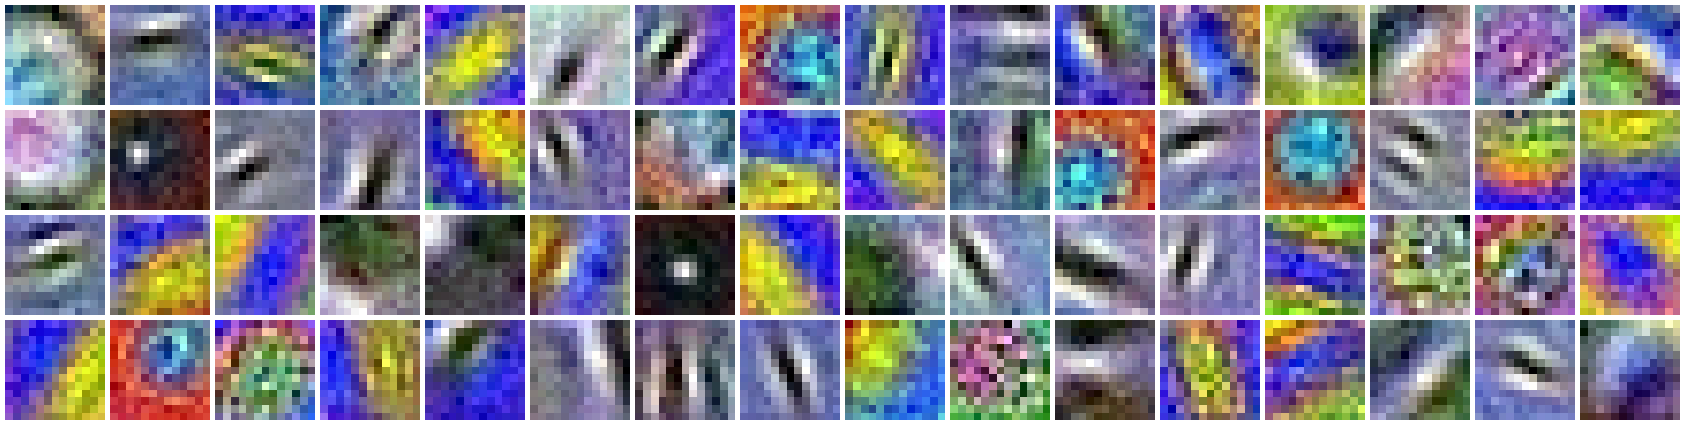
\includegraphics[width=1\columnwidth]{figs/network/Filter_unblurred.png}
\caption[Visualization of filter map]{Visualization of feature maps from the first convolutional layer of a trained network.}
\label{fig:convoluional_first_layer_visualization}
\end{center}
\end{figure}

Common for both convolutional layers and fully connected layers are the use of non-linear activation functions, which allow the network to learn non-linear decision boundaries. To compute the outgoing activation of any unit in the network, the incoming weights are first summed with the activations coming from either the input or the previous layer. Then, a bias is added, before feeding the result through the activation function. This is typically denoted:

$$ y = \sigma(aw + b),$$

\noindent where $a$ and  $w$ is \todo{are?} the unit's incoming activations and weights, $b$ is the bias and $\sigma$ is the non-linear activation function.\\

In the default hyperparameter configuration of this system, the output layer applies the logistic activation function, while the \ac{ReLU} activation function is used by the input and hidden layers. The logistic activation function is appropriate for the output layer, because it squashes any input to be between the value of 0 and 1. This is useful for the road detection system, where the activation of each output unit should predict a probability of whether the corresponding aerial image patch pixel belongs to the road class or not. The \ac{ReLU}, however, has been used for all other layers. This activation function has been shown to train deep neural networks faster. This non-linear activation function does not suffer from the gradient vanishing problem because it is non-saturating \citep{Krizhevsky_imagenet}. The activation functions are displayed in Figure \ref{fig:activation_functions}.\\

\begin{figure}[h]
\begin{subfigure}{0.45\textwidth}
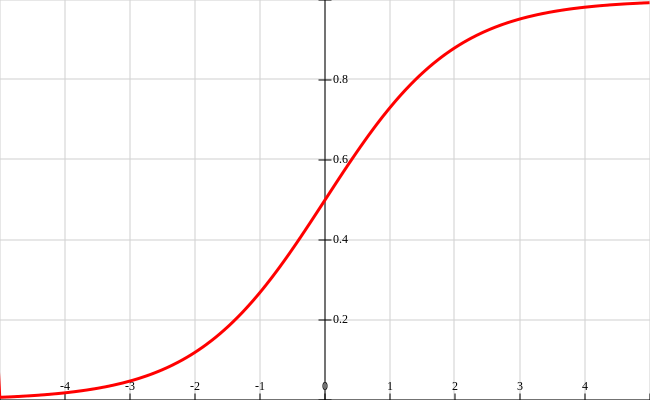
\includegraphics[width=\linewidth]{figs/sigmoid2.png}
$$ y = \frac{1}{1+ e^{-x}}$$
\caption{Logistic} \label{fig:activation_sigmoid}
\end{subfigure}
\hspace*{\fill} % separation between the subfigures
\begin{subfigure}{0.45\textwidth}
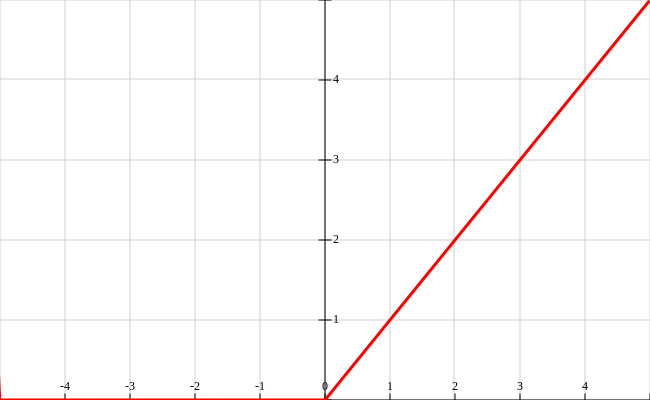
\includegraphics[width=\linewidth]{figs/relu2.png}
$$ y = \text{max}(0, x) \frac{}{}$$
\caption{Rectified linear unit} \label{fig:activation_relu}
\end{subfigure}
\hspace*{\fill} % separation between the subfigures
\caption[Activation functions]{Activation functions.} \label{fig:activation_functions}
\end{figure}


The specific network configuration values described in this section is the default configuration used in experiments found in Chapter \ref{cha:ResearchAndResults}. However, the network architecture can easily be changed through a configuration file. All configurable parameters related to the \ac{CNN} and their default values are listed in Table \ref{tab:network_parameters}.\\

\begin{table}[htp]
\caption[Hyperparameters for the CNN]{Hyperparameters for the \ac{CNN}.}
\begin{center}
\begin{adjustbox}{max width=\textwidth}
\begin{tabular}{+l ^p{5.5cm} ^l}\hline
\rowstyle{\bfseries}
  Parameter & Description & Value\\\hline
  $K^{(l)}$ & Number of kernels for convolutional layer $l$ & 64, 112, 80 \\
  $CLF^{(l)}$ & Filter size of convolutional layer $l$ & (13,13),(4,4),(3,3) \\
  $CLS^{(l)}$ & Stride size of convolutional layer $l$ & (4,4),(1,1),(1,1) \\
  $CLP^{(l)}$ & Pool size of convolutional layer $l$ & (2,2),(1,1),(1,1) \\
  $\mathcal{L}$ & Loss function  & Cross-entropy \\
  Epochs & How many epochs of training & 100 \\
  $\sigma^{(l)}$ & Activation function for each layer $l$ & ReLU x4, sigmoid x1 \\
  $h$ & Number of neurons in hidden layer & 4096 \\
  $p^{(l)}$ & Dropout rate for layer $l$ & 1.0, 0.9, 0.8, 0.5, 1.0 \\
  $ES_{init}$  & Initial early stopping patience in iterations & 100 000 \\
  $ES_{inc}$ & Increase factor for patience & 2 \\
  $ES_{thres}$  & Necessary improvement of validation loss before increasing patience & 0.997 \\
  $a$ & Learning rate & 0.0014 \\
  $a_{decrease}$ & learning rate decrease factor & 0.95 \\
  $\lambda$ & L2 weight decay strength & 0.0001 \\
  $m$ & Momentum & 0.9 \\
  $b$ & Batch size & 64 \\\hline
\end{tabular}
\end{adjustbox}
\end{center}
\label{tab:network_parameters}
\end{table}


\subsection{Optimization}
%\url{http://cs231n.github.io/neural-networks-3/}
%http://www.cs.toronto.edu/~tijmen/csc321/slides/lecture_slides_lec6.pdf}
%http://arxiv.org/pdf/1212.0901v2.pdf
%http://stats.stackexchange.com/questions/179915/whats-the-difference-between-momentum-based-gradient-descent-and-nesterovs-ac
The model parameters are optimized with a special form of \ac{SGD}, called Nesterov's accelerated gradient descent, and has an improved stability and faster convergence compared to standard \ac{SGD} \citep{Bengio_advances_optimizing}. The standard momentum approach extends the gradient update step by introducing velocity. The loss can be interpreted as a hilly error surface, where loss optimization can be viewed as a ball gaining and losing velocity while interacting with the landscape. When the loss optimization has gained velocity, it will stop doing purely steepest decent, which results in a smoother decent with fewer oscillations. Basically, instead of directly using the gradient to move in the landscape, the gradient will influence the velocity. The only hyperparameter associated with momentum is the decay coefficient $m$, which damps the velocity. \\


Nesterov momentum is a variation of momentum. Unlike standard momentum, the Nesterov method first makes a step in the direction of the accumulated velocity, and then makes a correction of the velocity based on the new location. In standard momentum, a correction to the velocity is made before taking a step. The Nesterov gradient is defined by the following update rule:

\begin{flalign*}
     &v_{t} = mv_{t-1} - a \nabla f(\theta_{t-1} + m v_{t-1}) \\
     &\theta_{t} = \theta_{t-1} + v_t,
\end{flalign*}

\noindent where $\theta_t$ is the model parameters, $v_t$ the velocity, $m$ the momentum decay, $a$ the current learning rate, and $\nabla f(z)$ is the gradient.\\

An important hyperparameter for gradient descent optimization methods is the learning rate $a$. In this implementation, the learning rate is annealed over time by step decay. The learning rate is decreased in a regular interval of epochs by some factor $a_{decrease}$ during optimization. \\

The default loss function of the system is cross-entropy loss, which in the context of the patch-based approach is denoted:

\begin{flalign*}
  \mathcal{L}_{\text{cross-entropy}}(q,y) =&  - \frac{1}{w_m^2} \sum\limits_{i=1}^{w_m^2} [y_i \log(q_i) + (1 -y_i)\log(1-q_i)],  \\ 
 \end{flalign*}

\noindent where $q$ and $y$ are the prediction and label patch. Each of the patches has $w_m^2$ probabilities and label values, that are used for computing the element-wise cross-entropy. Cross-entropy loss is non-negative and moves towards 0 as the network improves at the task. Given a training label and a predicted output, the loss function measure how well a neural network fits the training data. In addition, the backpropagation computes gradients based on the output of this loss function. At each iteration of training, the loss is minimized by slightly adjusting the weights of the network in the direction of these gradients.\\

\subsection{Regularization}
To avoid overfitting the training data, and hopefully achieve better generalization, different regularization schemes are applied during optimization, such as L2 weight decay, early stopping, and dropout. The classifier's task is to learn the regularities found in the mappings between the data and labels in the training set. However, the training set also contains sampling errors and accidental patterns not relevant to the task at hand. Without regularization, a classifier will learn the useful, but also the erroneous regularities a bit too well, and can, therefore, start to overfit the data. \\

L2 regularization is a weight decay method which applies a loss function penalty to prevent weights in the network from growing large. This is achieved by adding an extra term, $\lambda\sum_{i=0}^{|w|} w_i^2$ to the loss function, which penalizes large valued weights, and encourages a smoother parameter configuration \citep{Hinton_regularization}. The strength of the weight decay is controlled by the $\lambda$ hyperparameter, which is often set to a low value.\\

Early stopping interrupts the optimization process when performance on the validation set starts to consistently decrease. When the validation loss stagnates or starts to increase in value, the method waits for a certain number of iterations before stopping the training process. There are three parameters that control the early stopping behavior, $ES_{init}$, $ES_{thres}$, and $ES_{inc}$. The first parameter controls how many iterations the training should run for, regardless of validation loss performance. The second parameter dictates the required amount of improvement of the current validation loss compared to the best previously seen validation loss, before incrementing the patience variable. The latter parameter decides the increment factor of the patience. The patience is first initialized to wait for $ES_{init}$ iterations. If there is an improvement of validation loss above the $ES_{thres}$, the patience is set by  $\textit{patience} = max(\textit{patience}, \textit{iteration} \times ES_{inc} )$.\\
%http://link.springer.com/chapter/10.1007/3-540-49430-8_3

The dropout method forces the units to rely less on each other by randomly disabling units in the network during training. This encourages units to encode independently useful information, since dropout penalizes co-adaptation between units \citep{Srivastava_dropout}. Dropout can also be viewed as an ensemble method approximation. By randomly removing subsets of units from the network, an exponential number of parameter sharing subnetworks are trained simultaneously. This is less computationally expensive than training an ensemble of many individual deep neural networks. At test time, the predictions of these subnetworks are combined by an approximate averaging method. This is done by having the neural network produce predictions without dropping any units. Because all units make a contribution at test time, the weights of the network have to be scaled down. If a unit is retained with a probability of $p$ during training, the outgoing weights of that unit should be multiplied by $p$ at test time. Each layer $l$ has a unique dropout rate parameter $p^{(l)}$, which controls the probability of dropping a unit at that layer.  In the \ac{CNN} implementation, dropout has been implemented with some minor tweaks:

\begin{flalign*}
     &y = \frac{1}{p^{(l)}} r\circ \sigma(W^{(l)}x + b^{(l)}),
\end{flalign*}

\noindent where $W$ and $b$ are the weights and biases of layer $l$, $x$ denotes the input potentials, and $\sigma(z)$ is the activation function. $r$ is a vector of independent Bernoulli random variables, each having a probability of $p^{(l)}$ being 1 (and otherwise 0). The element-wise multiplication of this vector and the output vector of $\sigma(z)$, causes the activation of randomly picked units to be nullified. These units are essentially dropped out. Instead of scaling the outgoing weights at test time, the output activations are divided by $p^{(l)}$  during training, which should essentially give the same scaling effect.\\


\subsection{Data Preprocessing}
The datasets used in this thesis contains aerial images and road label maps that are very large. Each image is typically around $1500 \times 1500$ pixels in size, which is arguably too large for the model to use directly as input. Smaller patches of examples are therefore extracted from these larger images. From each image, a certain number of data patches and label patches of $64 \times 64$ and $16 \times 16$ are extracted randomly and added to a patch dataset.\\

However, before extracting patches, each aerial image and road label map pair is rotated by a random number of degrees between 0 and 360 degrees. This is necessary because of orientation bias in the datasets. In many cities, the road network is often constructed in a grid pattern, which leads to roads having certain orientations more often than not. Without random rotations of the training data, the model might become better at detecting roads only at certain orientations \citep{Mnih_roads_high_res_aerial_images}. Each image is therefore rotated by a random angle before extracting patches, which results in a patch training set that encourages the model to learn invariance to road orientation.\\

Another data augmentation method utilized when constructing the patch training set is flipping. This is a commonly used method to artificially increase the size of the dataset \citep{Krizhevsky_imagenet}. Since the dataset contains aerial imagery that depicts landscape from a top-down perspective, the patches can both be flipped vertically and horizontally.\\

Contrast normalization is also applied to every patch. Each patch is normalized by subtracting the mean pixel value from the pixels of the patch. The result is then divided by the standard deviation found for all pixels in the dataset.\\

Additionally, the datasets exhibit some class imbalance \citep{Japkowicz_class_imbalance}, which can be problematic since the optimization might prioritize loss minimization of classes that frequently occur in the training set and ignore rare classes. Random sampling of the patch datasets leads to a large imbalance between road examples and non-road examples. According to the label maps, the proportion of patches containing any road pixels, ranges between around 8\% and 25\%, depending on the dataset. This is solved by artificially increasing the proportion of road examples when sampling the patch dataset. Normally, a distribution of around 50\% road patches and 50\% non-road patches are used. However, this method is not applied to the test and validation patch set, which means that these sets will retain their natural class distribution. In Table \ref{tab:label_percentage} the percentage of road pixels for each dataset is listed. \\

\begin{table}[htp]
\caption[Percentage of road pixels in the dataset]{Percentage of road pixels in the datasets used by this thesis.}
\begin{center}
\begin{adjustbox}{max width=\textwidth}
\begin{tabular}{+l ^r ^r ^r}\hline
\rowstyle{\bfseries}
 		 Set & Massachusetts & Norwegian Vbase & Norwegian N50\\\hline
 		 Test & 4.70 & 4.60 & 2.76 \\
 		 Validation & 6.90  & 4.06 & 2.45 \\
 		 Training & 4.77 & 4.60 &  2.78\\\hline
\end{tabular}
\end{adjustbox}
\end{center}
\label{tab:label_percentage}
\end{table}